% Indicate the main file. Must go at the beginning of the file.
% !TEX root = ../main.tex

%%%%%%%%%%%%%%%%%%%%%%%%%%%%%%%%%%%%%%%%%%%%%%%%%%%%%%%%%%%%%%%%%%%%%%%%%%%%%%%%
% 04_results
%%%%%%%%%%%%%%%%%%%%%%%%%%%%%%%%%%%%%%%%%%%%%%%%%%%%%%%%%%%%%%%%%%%%%%%%%%%%%%%%

\section{Results}
\label{results}

    \subsection{Detection}

    - after detection how many sequences are excluded

    - how many images are left per label

    \subsection{Classification Performance}

    All classification models did perform well on the respective test sets.
    The balanced accuracy scores for each model are shown in \autoref{tab:bal_acc_by_model}.
    The pretrained models did perform better than the models trained from scratch which is demonstrated in \autoref{fig:bal_acc_img}.
    Generally the smaller models did perform a little better than the larger models but the differences are within the standard deviation.
    The pretrained EfficientNetB0 model achieved the highest balanced accuracy of 0.992 and a standard deviation of 0.004.
    The sequence classification applied to the image classification output did improve the balanced accuracy in all cases.
    Anyhow the improvement was in the range of 0.001 to 0.005 which is again within the standard deviation.

    %==== table: overview_dataset ====%
    \begin{table}[H]
\centering
\caption{Balanced accuracy of all models -- shown as mean ± standard deviation.}
\label{tab:bal_acc_by_model}
\begin{tabular}{l c r c c}
\toprule
Model & Pretrained & Params (M) & Image BA-Score & Sequence BA-Score \\
\midrule
efficientnet\_b0 & Yes & 4 & 0.9921 ± 0.004 & 0.9947 ± 0.002 \\
densenet169 & Yes & 12 & 0.9904 ± 0.004 & 0.9939 ± 0.002 \\
resnet50 & Yes & 23 & 0.9899 ± 0.004 & 0.9934 ± 0.002 \\
vit\_b\_16 & Yes & 85 & 0.9885 ± 0.005 & 0.9933 ± 0.002 \\
\midrule
efficientnet\_b0 & No & 4 & 0.9856 ± 0.005 & 0.9898 ± 0.003 \\
densenet169 & No & 12 & 0.9863 ± 0.006 & 0.9899 ± 0.002 \\
resnet50 & No & 23 & 0.9850 ± 0.004 & 0.9888 ± 0.003 \\
vit\_b\_16 & No & 85 & 0.9767 ± 0.006 & 0.9856 ± 0.004 \\
\bottomrule
\end{tabular}
\end{table}
    %=================================%

    \begin{figure}[ht]
    \centering
    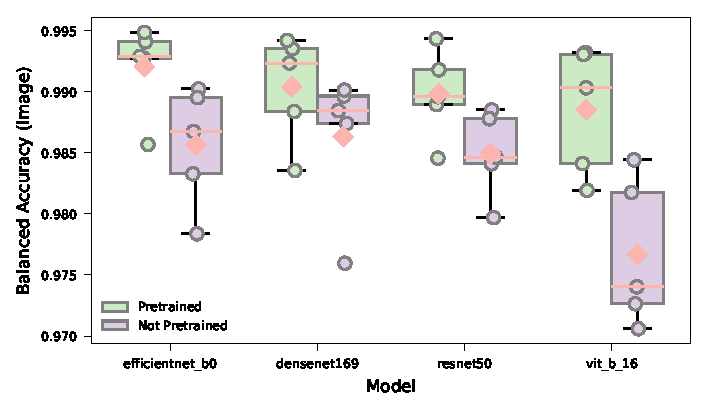
\includegraphics{figures/bal_acc_img.pdf}
    \caption{Balanced accuracy per model on the image level.}
    \label{fig:bal_acc_img}
    \end{figure}


    \subsection{Best Model}

    - More information on the best model including CM